\hypertarget{ch:probability}{%
\chapter{Probability and Paradoxes}\label{ch:probability}}

\hypertarget{probability}{%
\section{Probability}\label{probability}}

The world is random. Probability theory has been used to quantify the
randomness. We will go through examples to see how probability helps
interpret phenomena in real life and how probability may counter
intuition.

Some concepts:
\begin{itemize}
\item Experiment: a situations in which the outcome occur randomly.
\item Sample Space: the set of all possible outcomes in an experiment.
\item Event: a subset of the sample space is called an event; an event
  occur if the outcome from an experiment belong to the event.
\item Probability: assuming the elements of the sample space all have
  equal chance to occur, the probability of event $A$ is\\
  \begin{equation*}
    P(A)=\frac{n}{N}
    =\frac{\text{number of elements in A}}{\text{total number of outcomes}},
  \end{equation*}
  where \(n\) is the number of elements in \(A\) and \(N\) is the
  number of elements in the sample space.  Note that this formula
  holds only if all the outcomes are equally likely.
\end{itemize}

\hypertarget{example-elevator-waiting-time}{%
  \section{Elevator waiting
    time}\label{example-elevator-waiting-time}}

Mr. Smith works on the 13th floor of a 15 floor building. The only
elevator moves continuously through floors 1, 2, . . . 14, 15, 14,
. . . 2, 1, 2, . . . , except that it stops on a floor on which the
button has been pressed. Assume that time spent loading and unloading
passengers is very small compared to the travelling time.  Mr.~Smith
complains that at 5pm, when he wants to go home, the elevator almost
always goes up when it stops on his floor. What is the explanation?

There are 12 floors below the 13th floor and 15 floors above it, so the probability that the elevator is below the 13th floor is $12/14\approx0.86>0.5$. Thus no matter when Mr. Smith wants to go home, it is more likely that the elevator is going up.

We can simulate this situation:

\begin{knitrout}
\definecolor{shadecolor}{rgb}{0.969, 0.969, 0.969}\color{fgcolor}\begin{kframe}
\begin{alltt}
\hlkwd{set.seed}\hlstd{(}\hlnum{123}\hlstd{)} \hlcom{## set the random seed so that results are reproducible}
\hlstd{n} \hlkwb{<-} \hlnum{10000} \hlcom{## number of days to simulate}
\hlcom{## the sample space is the possible locations of the elevator [1, 15]}
\hlstd{elevator} \hlkwb{<-} \hlkwd{runif}\hlstd{(n,} \hlkwc{min}\hlstd{=}\hlnum{1}\hlstd{,} \hlkwc{max}\hlstd{=}\hlnum{15}\hlstd{)} \hlcom{## outcomes of experiments}
\hlstd{up} \hlkwb{<-} \hlstd{(elevator} \hlopt{<} \hlnum{13}\hlstd{)}
\hlcom{## the elevator is below the 13th floor so that it will goes up}
\hlkwd{sum}\hlstd{(up)} \hlopt{/} \hlstd{n}
\end{alltt}
\begin{verbatim}
## [1] 0.8633
\end{verbatim}
\end{kframe}
\end{knitrout}


\hypertarget{birthday-problem}{%
  \section{Birthday Problem}\label{birthday-problem}}

Suppose that a room contains 23 people. What is the probability that
at least two of them have a common birthday? Since each year has 365
days, this probability seems very small, but it is actually about
0.5. What is the probability that some one in that room has the same
birthday as yours? This probability is quite small
($\approx0.061$). In order to have the probability that someone's
birthday is the same as yours, we need 253 random selected people to
be in that room.

Let's use s simulation to verify the aforementioned numbers.

% \begin{equation*}
%   P(A)=1-P(A^c)=1-\frac{P_{365,n}}{365^n}=1-\frac{365\times364\times\cdots\times(365 - n + 1)}{365^n}
% \end{equation*}
% Some numbers:\\
% \begin{tabular}{lrrrrrr}\hline
%   $n$ & 4 & 16 & 23 & 32 & 40 & 56 \\
%   \hline
%   $P(A)$ & .016 & .284 & .507 & .753 & .891 & .988 \\\hline
% \end{tabular}
% \begin{equation*}
%   P(A)=1-P(A^c)=1-\frac{364^n}{365^n}
% \end{equation*}


\hypertarget{the-two-child-problem}{%
\section{The Two Child Problem}\label{the-two-child-problem}}


\hypertarget{simpsons-paradox}{%
\section{Simpson's Paradox}\label{simpsons-paradox}}

It is a phenomenon in which a trend appears in several different
groups of data but disappears or reverses when these groups are
combined.

\textbf{An urn example}: A black urn contains 5 red and 6 green balls,
and a white urn contains 3 red and 4 green balls. You are allowed to
choose an urn and then choose a ball at random from the urn. If you
choose a red ball, you get a prize. Which urn should you choose to
draw from?

\begin{itemize}
\item If you draw from the black urn, the probability of choosing a
  red ball is 5/11 = .455
\item If you choose to draw from the white urn, the probability of
  choosing a red ball is 3/7 = .429.
\end{itemize}

You should choose to draw from the black urn.

Now consider another game in which a second black urn has 6 red and
3 green balls, and a second white urn has 9 red and 5 green balls.

\begin{itemize}
\item If you draw from the black urn, the probability of a red ball is
  6/9 = .667
\item if you choose to draw from the white urn, the probability if
  9/14 = .643.
\end{itemize}

Again you should choose to draw from the black urn.

In the final game, the contents of the second black urn are added to
the first black urn, and the contents of the second white urn are
added to the first white urn. Again, you can choose which urn to draw
from. Which should you choose?

Intuition says choose the black urn, but let's calculate the
probabilities.

\begin{itemize}
\item The black urn now contains 11 red and 9 green balls, so the
  probability of drawing a red ball from it is 11/20=0.55
\item The white urn now contains 12 red and 9 green balls, so the
  probability of drawing a red ball from it is 12/21= .571.
\end{itemize}

You should choose the white urn!

\textbf{UC Berkeley gender bias:} A famous example of Simpson's
paradox is a study of gender bias among graduate school admissions to
University of California, Berkeley. In 1973 UC Berkeley was sued for
sex-discrimination. Here are the overall numbers for the six largest
departments in fall admission of 1973.

\begin{center}
\begin{tabular}{crrcrr}\hline
 \multicolumn{3}{c}{Men} & \multicolumn{3}{c}{Women} \\\hline
 Applicants & \multicolumn{2}{c}{Admitted}     & Applicants & \multicolumn{2}{c}{Admitted} \\\hline
 2691       & 1198 & ({\bf 44.5}\%) & 1835       & 557 & (30.4\%) \\\hline
\end{tabular}
\end{center}

This table shows that men were more likely than women to be admitted,
and the difference was so significant. Let's see which departments
were mainly responsible for this gender bias. To do this we broke open
the data according to each departments.

\begin{center}
\begin{tabular}{ccrrcrr}\hline
  & \multicolumn{3}{c}{Men}  & \multicolumn{3}{c}{Women} \\\cline{2-7}
Department & Applicants  & \multicolumn{2}{c}{Admitted} & Applicants  & \multicolumn{2}{c}{Admitted} \\\hline
A & 825 & 512& (62\%) & 108 & 89 &(82\%)  \\ 
B & 560 & 353& (63\%) & 25  & 17 &(68\%)  \\
C & 325 & 120& (37\%) & 593 & 202& (34\%) \\
D & 417 & 138& (33\%) & 375 & 131& (35\%) \\
E & 191 & 53 & (28\%) & 393 & 94 &(24\%)  \\
F & 373 & 22 & (6\%) & 341 & 24 &(7\%)  \\\hline
\end{tabular}
\end{center}

Things get strange after we divide the data according different departments. For the six departments, four of them accepted women more than men. 
To explain this, \cite{bickel1975sex} noticed that women tended to apply to more competitive departments with low admission rates even among qualified applicants, whereas men tended to apply to less competitive departments with high admission rates among the qualified applicants.

To use simulation to further illustrate this, we simulate a data set with four groups in the following.
\begin{knitrout}
\definecolor{shadecolor}{rgb}{0.969, 0.969, 0.969}\color{fgcolor}\begin{kframe}
\begin{alltt}
\hlkwd{set.seed}\hlstd{(}\hlnum{2021}\hlstd{)}
\hlstd{g} \hlkwb{<-} \hlnum{4} \hlcom{# number of groups}
\hlstd{n} \hlkwb{<-} \hlnum{40} \hlcom{# number of instances in each group}
\hlstd{z} \hlkwb{<-} \hlkwd{rep}\hlstd{(}\hlnum{1}\hlopt{:}\hlnum{4}\hlstd{,} \hlkwc{each}\hlstd{=n)} \hlcom{# grouping variable}
\hlstd{x} \hlkwb{<-} \hlkwd{runif}\hlstd{(n}\hlopt{*}\hlstd{g,} \hlnum{0}\hlstd{,} \hlnum{2}\hlstd{)} \hlopt{+} \hlstd{z} \hlcom{# x variable that depends on z}
\hlstd{y} \hlkwb{<-} \hlnum{2} \hlopt{*} \hlstd{z} \hlopt{-} \hlstd{x} \hlopt{+} \hlkwd{rnorm}\hlstd{(n}\hlopt{*}\hlstd{g)} \hlcom{# y variable that depends on x and z}
\hlkwd{plot}\hlstd{(x, y)} \hlcom{# plot the whole data}
\end{alltt}
\end{kframe}\begin{figure}

{\centering 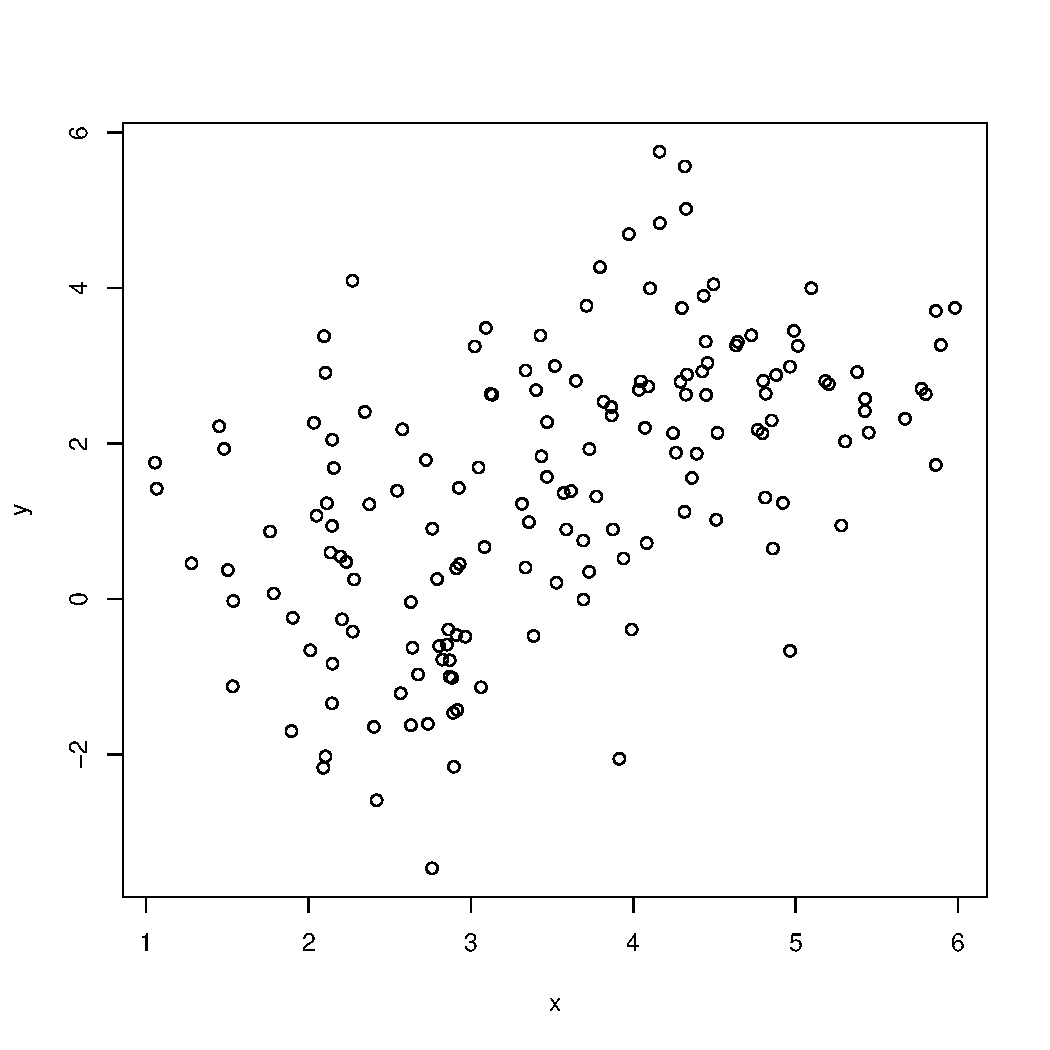
\includegraphics[width=\maxwidth]{figure/probability-Simpson-1} 

}

\caption[Scatter plot for the whole data]{Scatter plot for the whole data}\label{fig:probability-Simpson}
\end{figure}

\end{knitrout}

\begin{knitrout}
\definecolor{shadecolor}{rgb}{0.969, 0.969, 0.969}\color{fgcolor}\begin{kframe}
\begin{alltt}
\hlkwd{plot}\hlstd{(x, y,} \hlkwc{pch}\hlstd{=}\hlkwd{rep}\hlstd{(}\hlnum{1}\hlopt{:}\hlstd{g,} \hlkwc{each}\hlstd{=n),} \hlkwc{col}\hlstd{=}\hlkwd{rep}\hlstd{(}\hlnum{1}\hlopt{:}\hlstd{g,} \hlkwc{each}\hlstd{=n))}
\end{alltt}
\end{kframe}\begin{figure}

{\centering 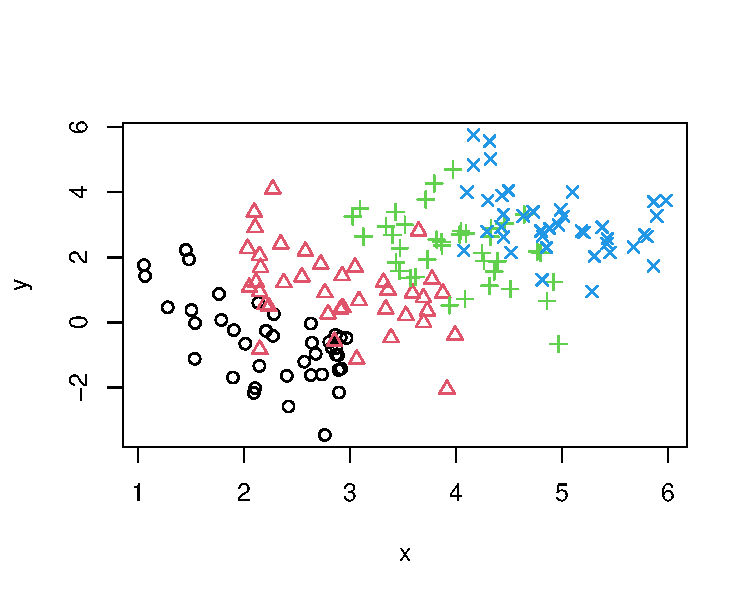
\includegraphics[width=\maxwidth]{figure/probability-Simpson2-1} 

}

\caption[Scatter plot with different groups labeled]{Scatter plot with different groups labeled}\label{fig:probability-Simpson2}
\end{figure}

\begin{kframe}\begin{alltt}
\hlcom{# label the points for different groups}
\end{alltt}
\end{kframe}
\end{knitrout}

We see that for the whole data, $y$ has an increase pattern as $x$ increases, but for each sub group $y$ has a decrease pattern as $x$ increases.

\hypertarget{prisoners-problem}{%
\section{100 prisoners problem}\label{prisoners-problem}}

%%% Local Variables:
%%% coding: utf-8
%%% mode: latex
%%% TeX-master: "00why.tex"
%%% End:

%%% TeX-engine: xetex
%%% TeX-command-extra-options: "-shell-escape"
